%************************************************************************************************************%
% This is a short introduction to the beamer class used by LaTex.  The beamer class allows you write LaTex   % 
% documents for presentations.                                                                               %
%************************************************************************************************************%

%----------------------------------Written by: Omair Zubairi @ SDSU------------------------------------------%


%++++++++++++++++++++++++++++++++++++++++++++++++++++++++++++++++++++++++++++++++++++++++++++++++++++++++++++%
% The author gives permission to download, modify, and to use this document as he/she pleases.  Note that    %
% this is only a guide to learn LaTex and how to use the Beamer class.  Many tutorials are available on      %
% the Web.  A good place to start is Wiki Books on LaTex                                                     %
%++++++++++++++++++++++++++++++++++++++++++++++++++++++++++++++++++++++++++++++++++++++++++++++++++++++++++++%



\documentclass{beamer}  % Define your document class
\usetheme{CambridgeUS}       % The Theme of your presentation (many others available on the web)
\usepackage{amsmath}
\usepackage{verbatim}
 

\title[Orbital Patterns of Martian Moons]{Orbital Patterns of Martian Moons}
\author{Jake Mathews \& Ian Brown}
\institute{Wentworth Institute of Technology}
\date{August 6th, 2018}


%Actual code starts here---
\begin{document}

\begin{frame}
\titlepage
\end{frame}


% Here is a Frame 1------------------------------------------------------------------------------------------------
\begin{frame}{Outline} % Frame title

% Bullet points...
 \begin{itemize}
  \item Model Goals
  \item Problem Overview
  \item Calculations
  \item Conclusion
  \item Sources \& Questions
 \end{itemize}

\end{frame}
%End Frame 1-------------------------------------------------------------------------------------------------------


% Here is a Frame 2------------------------------------------------------------------------------------------------
\begin{frame}{Model Goals} % Frame title
\begin{itemize}
	\item The goal of our project is to model the interactions of the moons Phobos \& Deimos with the planet Mars due to Gravity
	\item The program we created will simulate an objects path given some initial conditions and a gravitational constant. 
	\item The simulation is run for each moon to simulate their interactions with the planet.
\end{itemize}
\end{frame}

%Frame 3-----------------------------------------------------------------------------------------------------------
\begin{frame}{Problem Overview}

\begin{figure}
\label{fig:1}
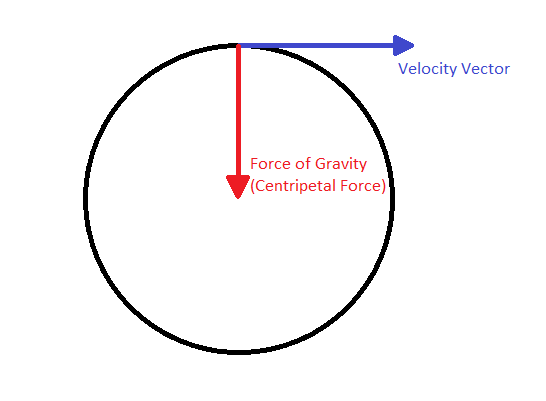
\includegraphics[scale=0.5]{orbitalDiagram}
\caption{Orbital Diagram}
\end{figure}

\end{frame}
%End Frame 3-------------------------------------------------------------------------------------------------------

%Frame 4-----------------------------------------------------------------------------------------------------------
\begin{frame}{Calculations}
Before performing the calculations to determine an objects new position in space, we must have some initial conditions to go off of. The initial conditions that need to be set are:

\begin{itemize}

\item Gravitational Constants for Phobos and Deimos
\begin{itemize}
\item Normalized for each moon
\end{itemize}

\item Initial Position (X and Y Positions)
\item Initial Velocity (X and Y Velocity Vectors)

\item Time
\begin{itemize}
\item Time Step
\item Initial Time
\item Orbital Period (Max Time)
\end{itemize}

\end{itemize}



\end{frame}
%End Frame 4------------------------------------------------------------------------------------------------------

%Frame 5-----------------------------------------------------------------------------------------------------------
\begin{frame}{Calculations - Initial Position}

\begin{itemize}
\item We set the initial position of each moon to be at the semi-major axis of their orbit.
\item The semi-major axis of each moon as defined by Nasa are:
\begin{itemize}
	\item Phobos: $9378km \rightarrow 9.378 x 10^6m$
	\item Deimos: $23459km \rightarrow 23.459 x 10^6m$
\end{itemize}
\end{itemize}

\begin{figure}
\label{fig:2}
\caption{Semi-Major Axis Illustration}
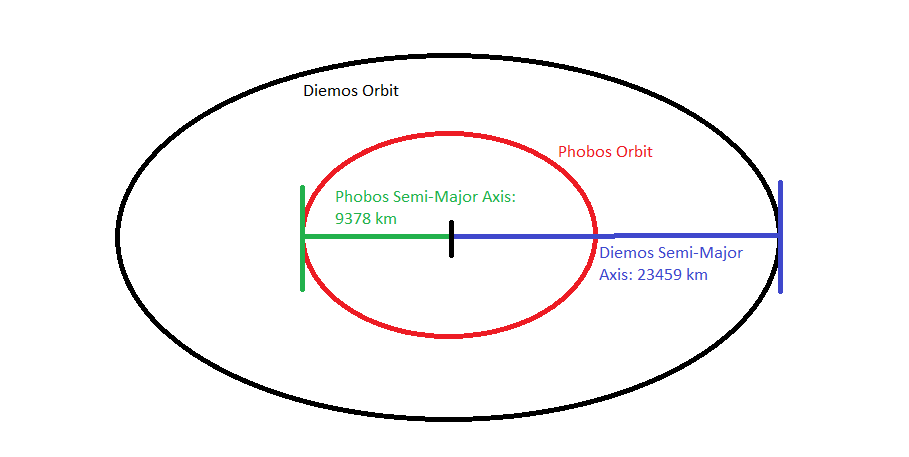
\includegraphics[scale=0.45]{semi-majorAxis}

\end{figure}


 \end{frame}
%End Frame 5-------------------------------------------------------------------------------------------------------

%Frame 6-----------------------------------------------------------------------------------------------------------
\begin{frame}{Calculations - Gravitational Constants}
The calculations will be simplified if we can normalize the gravitational constant for each moon.

\begin{columns} % here is where you begin your columns
 
 \begin{column}{0.50\textwidth} %first column with a defined size...
  \begin{block}{Phobos} % remember this is the block title...
   \begin{itemize}
   	\item $G = 6.683*10^(-11) N*m^2*kg^{-2}$
     \item $G = 4\pi ^{2}*\frac{R^{3}}{Year_{Phobos}*M_{System}}$
     \item $R =  9.378 x 10^6m$
	\item $M_{System} = M_{Mars} + M_{Phobos}$
	\item $M_{Phobos} = 10.6 * 10^{15} kg$
	\item $Year_{Phobos} = 27553.82 s$
	\item $Gravity_{Phobos} = 4.2887 * 10^{13}$
   \end{itemize}
  \end{block}
 \end{column}

 \begin{column}{0.50\textwidth} % second column  
  \begin{block}{Deimos}
   \begin{itemize}
     \item $G = 6.683*10^(-11) N*m^2*kg^{-2}$
     \item $G = 4\pi ^{2}*\frac{R^{3}}{Year_{Moon}*M_{System}}$
     \item $R =  23.459 x 10^6m$
	\item $M_{System} = M_{Mars} + M_{Moon}$
	\item $M_{Diemos} = 2.4 * 10^{15} kg$
	\item $Year_{Diemos} = 109074.81 s$
	\item $Gravity_{Phobos} = 4.2839  10^{13}$
   \end{itemize}
  \end{block}
 \end{column}

\end{columns}

 \end{frame}
%End Frame 6-------------------------------------------------------------------------------------------------------

%Frame 7-----------------------------------------------------------------------------------------------------------
\begin{frame}{Calculations - Initial Velocity}
Now that we have normalized the gravitational constants, determining each moons initial velocity

\begin{columns} % here is where you begin your columns
 
 \begin{column}{0.50\textwidth} %first column with a defined size...
  \begin{block}{Phobos} % remember this is the block title...
   \begin{itemize}
   	\item $F=ma$
	\item $F_{Net}=\frac{M_{Phobos}*v^{2}}{R}$
	\item $F_{Gravity}=\frac{G_{Phobos}}{R^{2}}$
	\item $F_{Net} = F_{Gravity}$
     \item $V_{Phobos} = \sqrt{\frac{Gravity_{Phobos}}{R_{Phobos}}}$
   \end{itemize}
  \end{block}
 \end{column}

 \begin{column}{0.50\textwidth} % second column  
  \begin{block}{Deimos}
   \begin{itemize}
     \item $F=ma$
	\item $F_{Net}=\frac{M_{Deimos}*v^{2}}{R}$
	\item $F_{Gravity}=\frac{G_{Deimos}}{R^{2}}$
	\item $F_{Net} = F_{Gravity}$
     \item $V_{Deimos} = \sqrt{\frac{Gravity_{Deimos}}{R_{Deimos}}}$
   \end{itemize}
  \end{block}
 \end{column}

\end{columns}

\end{frame}
%End Frame 7-------------------------------------------------------------------------------------------------------

%Frame 8-----------------------------------------------------------------------------------------------------------
\begin{frame}{Calculations - Time}

\begin{itemize}
	\item Time Step
	\begin{itemize}
		\item A time step ($deltaTime = dt$) will be 1 second increments ($dt = 1.0s$)
	\end{itemize}
	\item Initial Time
	\begin{itemize}
		\item $t = 0.0s$
	\end{itemize}
	\item Orbital Periods are constants retrieved from Nasa
	\begin{itemize}
		\item Phobos: $tmax = 27553.824s$
		\item Deimos: $tmax = 109074.816s$
	\end{itemize}
\end{itemize}

\end{frame}
%End Frame 8-------------------------------------------------------------------------------------------------------

%Frame 9-----------------------------------------------------------------------------------------------------------
\begin{frame}{Calculations - Fourth Order Runge Kutta Method}

\begin{columns} % here is where you begin your columns

 \begin{column}{0.50\textwidth} %first column with a defined size...
  	\begin{block}{Right Hand Rule} 
   		 \begin{itemize}
     		 \item $\sum_{t=0}^{year}y(t)*dt$
   		 \end{itemize}
   	\end{block}
	
	\begin{block}{RK4 Expressions} % remember this is the block title...
    \begin{itemize}
      \item $k_{1}= \Delta t\vec{f}(\vec{y}^{n},t)$
      \item $k_{2}= \Delta t\vec{f}(\vec{y}^{n} + \frac{1}{2}k_{1},t + \frac{1}{2}\Delta t)$
      \item $k_{3}= \Delta t\vec{f}(\vec{y}^{n} + \frac{1}{2}k_{2},t + \frac{1}{2}\Delta t)$
      \item $k_{4}= \Delta t\vec{f}(\vec{y}^{n} + k_{3}, t + \Delta t)$
    \end{itemize}
  \end{block}
 \end{column}

 \begin{column}{0.50\textwidth} % second column  

\begin{figure}
\label{fig:3}
\caption{Runge Kutta}
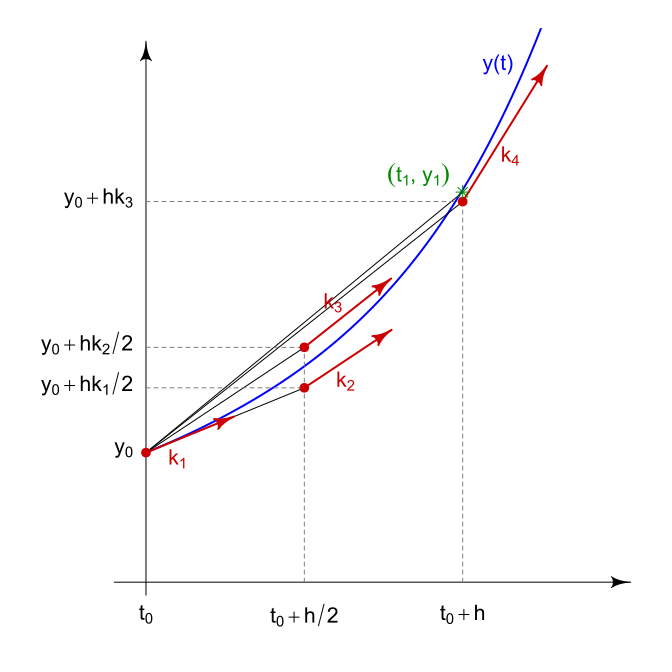
\includegraphics[scale=0.35]{runge-kutta}
\end{figure}
 \end{column}
\end{columns}

\end{frame}
%End Frame 9-------------------------------------------------------------------------------------------------------

%Frame 11-----------------------------------------------------------------------------------------------------------
\begin{frame}{Conclusion}

\end{frame}
%End Frame 11-------------------------------------------------------------------------------------------------------

%Frame 10-----------------------------------------------------------------------------------------------------------
\begin{frame}{Calculations - Fourth Order Runge Kutta Method}

  \begin{block}{RK4} % remember this is the block title...
    \begin{itemize}
      \item $k_{1}= \Delta t\vec{f}(\vec{y}^{n},t)$
      \item $k_{2}= \Delta t\vec{f}(\vec{y}^{n} + \frac{1}{2}k_{1},t + \frac{1}{2}\Delta t)$
      \item $k_{3}= \Delta t\vec{f}(\vec{y}^{n} + \frac{1}{2}k_{2},t + \frac{1}{2}\Delta t)$
      \item $k_{4}= \Delta t\vec{f}(\vec{y}^{n} + k_{3}, t + \Delta t)$
    \end{itemize}
  \end{block}

\end{frame}
%End Frame 10-------------------------------------------------------------------------------------------------------

%Frame 11-----------------------------------------------------------------------------------------------------------
\begin{frame}{Sources and Questions}

\begin{itemize}
	\item "Riemann Sum." Low-Pass Filter - Howling Pixel, \url{howlingpixel.com/i-en/Riemann_sum}
\end{itemize}

\end{frame}
%End Frame 11-------------------------------------------------------------------------------------------------------


\end{document} %Document ends here...